% !TeX program = lualatex
% ================================================================
% Polish Parallel Text Version of VectorChallengeSheet
%
% Generated by the server using the following settings:
%
%   language            Polish (pol)
%   text direction      left to right
%   font                Noto Serif
%   fallback font       Noto Serif
%   built from          latex/worksheets/geometry/vectors/vectorChallengeSheet.tex
%   vocabulary key      latex/worksheets/geometry/vectors/vectorChallengeSheet/L2/pol/vectorChallengeSheet_polishKey.tex
%   tier 3 vocabulary   green   RGB 0 128 0
%   English text        black   RGB 0 0 0
%   Polish text         purple  RGB 112 48 160
%   layout macros       version 3
%
% Please don't edit any information in this comment block - the server
% compares it against the current settings and rebuilds this file when
% they differ, so changes here would be overwritten. However, feel free
% to make updates to the LaTeX below if you want to edit it.
% ================================================================

\documentclass[20pt]{ctexart}
% ================================================================
% Copied from the English sheet this was translated from, so that
% anything it sets up for itself still works here
% ================================================================
\usepackage{amsmath, amssymb}
\usepackage{tikz}
\usepackage{geometry}
\usepackage{booktabs}
\usepackage{enumitem}
\geometry{margin=1in}
\usetikzlibrary{arrows.meta}

 \newgeometry{left=0.5cm,bottom=0.1cm}


\newcommand{\overarrow}[1]{\overrightarrow{#1}}
\newcommand{\colvec}[2]{\begin{pmatrix} #1 \\ #2 \end{pmatrix}}

\title{Vectors, Translations, and Meaning}
\author{Extension Sheet}
\date{}

% Characters this language's font has not got are borrowed from another,
% rather than being silently dropped - see docs/translated-sheet-latex.md
\directlua{%
  if luaotfload and luaotfload.add_fallback then
    luaotfload.add_fallback("eallatinfallback",
      { "Noto Serif:mode=harf;" })
  else
    tex.error("this luaotfload is too old to register a fallback font")
  end
}
\usepackage[english]{babel}
\babelprovide[import]{polish}
\babelfont[polish]{rm}[Renderer=Harfbuzz, BoldFont={Noto Serif}, ItalicFont={Noto Serif}, BoldItalicFont={Noto Serif}, RawFeature={fallback=eallatinfallback}]{Noto Serif}
\babelfont[polish]{sf}[Renderer=Harfbuzz, BoldFont={Noto Serif}, ItalicFont={Noto Serif}, BoldItalicFont={Noto Serif}, RawFeature={fallback=eallatinfallback}]{Noto Serif}
\newcommand{\ealtext}[1]{\foreignlanguage{polish}{#1}}
\newcommand{\ealtextblock}[1]{{\raggedright\foreignlanguage{polish}{#1}\par}}
% ================================================================
% EAL layout helpers
% ================================================================
\usepackage{xcolor}

\definecolor{ealkeycolour}{RGB}{0,128,0}
\definecolor{ealenglish}{RGB}{0,0,0}
\definecolor{ealtwocolour}{RGB}{112,48,160}

\newsavebox{\ealboxen}
\newsavebox{\ealboxtr}
\newlength{\ealglosswd}
\newlength{\ealglossraise}
\setlength{\ealglossraise}{1.15em}

% a tier 3 word, in English and in translation alike
\newcommand{\ealkey}[1]{\textcolor{ealkeycolour}{#1}}
\newcommand{\ealkeytr}[1]{\textcolor{ealkeycolour}{\ealtext{#1}}}

% One translated word above one English word. Built from kernel
% primitives, never a tabular, which would break wherever the sheet
% loads array, booktabs or tabularx. The box is as wide as the wider of
% the two, so a long translation pushes its neighbours aside instead of
% overlapping them, and it claims its full height so a table row or a
% TikZ node makes room for it.
\newcommand{\ealgloss}[2]{%
  \sbox{\ealboxen}{\ealkey{#1}}%
  \sbox{\ealboxtr}{\small\textcolor{ealtwocolour}{\ealtext{#2}}}%
  \setlength{\ealglosswd}{\wd\ealboxen}%
  \ifdim\wd\ealboxtr>\ealglosswd\setlength{\ealglosswd}{\wd\ealboxtr}\fi
  \leavevmode
  \makebox[\ealglosswd][c]{%
    \makebox[0pt][c]{\usebox{\ealboxen}}%
    \makebox[0pt][c]{\raisebox{\ealglossraise}{\usebox{\ealboxtr}}}%
  }%
}

% opens up line spacing around a block of glosses, so the raised
% translations sit clear of the line above
\newenvironment{ealglossed}{\par\linespread{2.1}\selectfont\ignorespaces}{\par}

% a whole translated sentence above its English counterpart. block level,
% so it does not belong inside a tabular cell
\newcommand{\ealpara}[2]{%
  \par\addvspace{0.5\baselineskip}%
  {\color{ealtwocolour}\ealtextblock{#1}}%
  \penalty200
  {\color{ealenglish}#2\par}%
  \addvspace{0.5\baselineskip}%
}

\begin{document}
\maketitle

\section*{1\quad \ealkey{Vector} \ealkey{translation} review}

\ealpara{Punkt $A = (2,3)$ jest przesuwany o $ \bf{t}=\colvec{4}{1}$. Znajdź punkt końcowy.}{Point $A = (2,3)$ is translated by $ \bf{t}=\colvec{4}{1}$. Find the destination.}

\vspace{4em}

\ealpara{Zastosuj to samo \ealkeytr{przesunięcie} do $B = (-1,5)$.}{Apply the same \ealkey{translation} to $B = (-1,5)$.}

\vspace{5em}

\section*{2 \quad Word \ealkey{embeddings}}

\ealpara{Modele AI biorą słowa i przypisują im \ealkeytr{współrzędne} $(x,y)$, dzięki czemu słowa mogą być przetwarzane przez algorytmy - nazywa się to \textbf{\ealkeytr{osadzeniem} słów}. Poniżej znajduje się przykład tego dla 8 słów:}{AI models take words and assign them \ealkey{coordinates} $(x,y)$, so that the words can be processed by algorithms - this is called a \textbf{word \ealkey{embedding}}. Below is an example of this for 8 words:}

\begin{center}
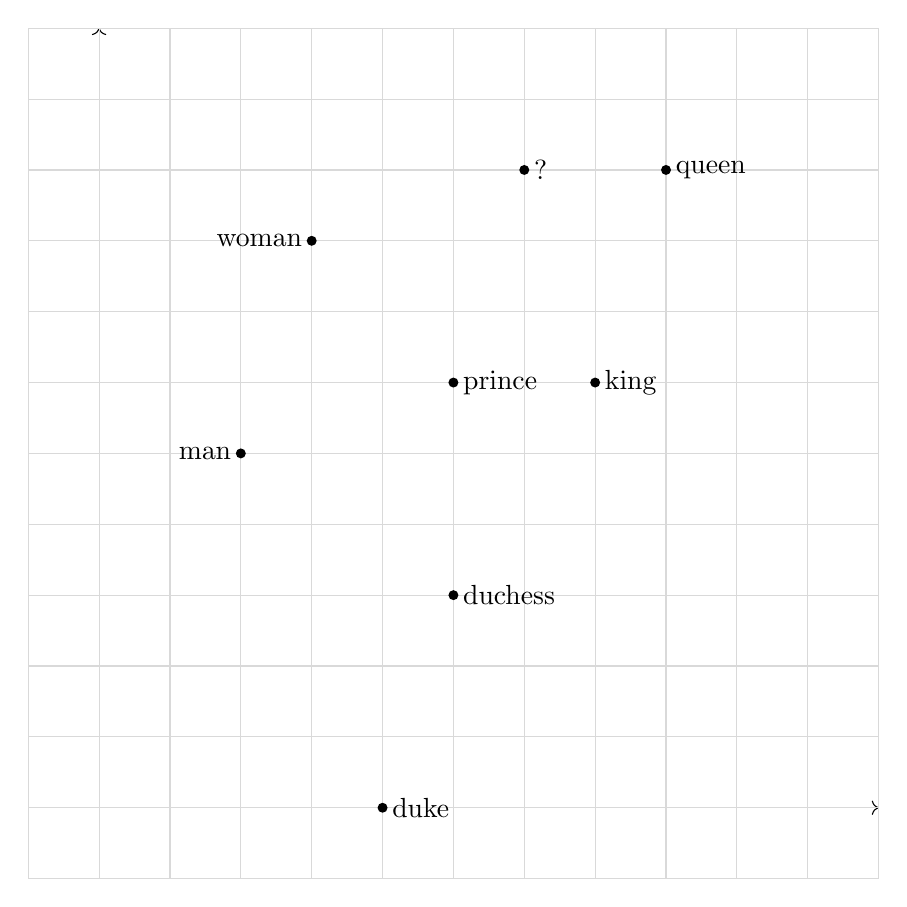
\begin{tikzpicture}[scale=0.9]
  % axes and grid
  \draw[->] (-1,0)--(11,0);
  \draw[->] (0,-1)--(0,11);
  \draw[step=1cm,gray!30] (-1,-1) grid (11,11);

  % semantic cluster (left side)
  \fill (2,5) circle (2pt) node[left] {man};
  \fill (3,8) circle (2pt) node[left] {woman};
  \fill (7,6) circle (2pt) node[right] {king};
  \fill (8,9) circle (2pt) node[right] {queen};
  \fill (5,6) circle (2pt) node[right] {prince};
  \fill (4,0) circle (2pt) node[right] {duke};
  \fill (5,3) circle (2pt) node[right] {duchess};

  % missing princess (dashed)
  \fill (6,9) circle (2pt) node[right] {?};

\end{tikzpicture}
\end{center}

\newpage{}

\begin{enumerate}[label=\textbf{\arabic*.}]
  \item \ealpara{Oblicz \ealkeytr{wektor} $\overarrow{\text{king}\quad\text{queen}}$.}{Compute the \ealkey{vector} $\overarrow{\text{king}\quad\text{queen}}$.} \vspace{5em}
  \item \ealpara{Oblicz \ealkeytr{wektor} $\overarrow{\text{duke} \quad\text{duchess}}$.}{Compute the \ealkey{vector} $\overarrow{\text{duke} \quad\text{duchess}}$.} \vspace{5em}

  \item \ealpara{Jak myślisz, co reprezentuje \ealkeytr{przesunięcie} $\colvec{1}{3}$ w naszym \ealkeytr{osadzeniu} \ealkeytr{wektorowym} słów?}{What do you think the \ealkey{translation} $\colvec{1}{3}$ represents in our word \ealkey{vector} \ealkey{embedding}?}

\vspace{5em}

  \item \ealpara{Rozważ $\overarrow{\text{man} \quad \text{woman}}$; czy zgadza się to z twoją odpowiedzią na poprzednie pytanie?}{Consider $\overarrow{\text{man} \quad \text{woman}}$, does that match up with your answer to the previous question?}

  \vspace{5em}

  \item \ealpara{Jakie słowo brakuje przy znaku zapytania?}{What word is missing at the question mark ?}
\end{enumerate}

\newpage{}
\section*{3 \quad Translating English to Chinese}

\ealpara{\ealkeytr{Przesunięcie} maszynowe to dziedzina AI, która zajmuje się tłumaczeniem tekstu między dwoma różnymi językami; poniżej znajduje się niekompletna siatka i tabela \ealkeytr{przesunięć}:}{Machine \ealkey{translation} is a field of AI that deals with translating text between two different languages, below is an incomplete grid and \ealkey{translation} table:}




\begin{center}

\begin{tikzpicture}[scale=0.65]
  \draw[step=1cm,gray!50] (-10,-10) grid (15,15);

  \draw[->] (-10,0)--(15,0);
  \draw[->] (0,-10)--(0,15);

  % English cluster
  \fill (9,8) circle (2pt) node[above right] {man};
  \fill (10,11) circle (2pt) node[above right] {?};

  \fill (7,8) circle (2pt) node[above right] {boy};
  \fill (8,11) circle (2pt) node[above right] {girl};
  \fill (8,6) circle (2pt) node[above right] {king};
  \fill (9,9) circle (2pt) node[above right] {?};

  \fill (6,6) circle (2pt) node[above right] {?};
  \fill (7,9) circle (2pt) node[above right] {?};


  % Chinese cluster (shifted)
  \fill (-6,-2) circle (2pt) node[right] {男人};
  \fill (-5,1) circle (2pt) node[right] {?};
  \fill (-6,-1) circle (2pt) node[right]  {王妃};
  \fill (-7,-4) circle (2pt) node[right] {国王};
  

  % gender pair in Chinese
  \fill (-8,-2) circle (2pt) node[right] {?};
  \fill (-7,1) circle (2pt) node[right] {女孩};

  \fill (-9,-4) circle (2pt) node[right] {王子};
  \fill (-9,0) circle (2pt) node[right] {?};



\end{tikzpicture}
\end{center}

\subsection*{\ealkey{Translation} table (incomplete)}

\begin{center}
\begin{tabular}{@{}llll@{}}
\toprule
English & English coords & Chinese & Chinese coords \\
\midrule
man     & (9,8)  & 男人 & (-6,-2) \\
woman & (10,11) & 女人 & (-5,1) \\
boy     &  & 男孩 &  \\
 &  & 女孩 & (-7,1) \\
 & (8,6)  & &  \\
 & & 王妃 &  \\
prince & & 王子 &  \\
princess & (7,9) & 公主 & (-9,0)  \\


\bottomrule
\end{tabular}
\end{center}



\subsection*{Tasks}

\begin{enumerate}[label=\textbf{\arabic*.}]

\item \ealpara{Użyj podanych \ealkeytr{współrzędnych} i tabeli, aby obliczyć \ealkeytr{wektor} \ealkeytr{przesunięcia} $\bf{t}$ z angielskiego na chiński.}{Use the given \ealkey{coordinates} and table to compute the \ealkey{translation} \ealkey{vector} $\bf{t}$ from English to Chinese.}

\vspace{5em}

\item \ealpara{Uzupełnij brakujące wartości w tabeli i siatce.}{Fill in the missing values in the table and coordinate grid}

\vspace{5em}

\item \ealpara{(Wyzwanie) Jak myślisz, co oznacza \ealkeytr{wektor} $\colvec{-2}{0}$ w kontekście tego \ealkeytr{osadzenia} \ealkeytr{wektorowego} słów?}{(Challenge) What do you think the \ealkey{vector} $\colvec{-2}{0}$ means in the context of this word-\ealkey{vector} \ealkey{embedding}?}

\vspace{5em}

\item \ealpara{(Wyzwanie) Dolny wiersz tabeli nie podąża za wzorem; jak myślisz, dlaczego tak jest? (wskazówka - rozważ chińskie znaki)}{(Challenge) The bottom row of the table does not follow the pattern, why do you think this is? (hint - consider the Chinese characters)}

\end{enumerate}

\bigskip

\newpage
\end{document}